\chapter{Einführung}\label{01_einf}
\thispagestyle{fancy}

In diesem Kapitel wird anhand der IT-Sicherheitsziele aufgezeigt, dass man unter dem 
Begriff Servicemonitoring auch immer den Begriff Securitymonitoring verstehen
kann. Auch soll darauf hingewiesen werden, dass der Ausdruck Überwachung im ganzen
Dokument mit der Bedeutung: Aufsicht oder Monitoring belegt wird um eine klare Abgrenzung
zur zweiten Bedeutung: Observation, Beschattung (engl. surveillance) zu erlangen.


\section{Servicemonitoring und Securitymonitoring}

Die Überwachung von Diensten ist mittlerweile ein integraler Bestandteil der 
Infrastruktur jedes IT-~Diensteanbieters geworden. Neben der einfachen Erfassung
und der (z.B. grafischen) Aufarbeitung verschiedenster Messgrößen, werden die erfassten 
Daten zunehmend analysiert und es wird versucht Muster zu erkennen. Dieser Vorgang wird 
auch als \textit{BigData} bezeichnet. Diese Daten werden auch verstärkt zur 
Sicherheitsanalyse herangezogen. Daher stellt sich die Frage, ob Securitymonitoring 
äquivalent zum Servicemonitoring - Begriff ist. Um es vorweg zunehmen, ja, denn es kommt 
ausschließlich auf die Fragestellung an, die man mit den erfassten Daten klären möchte. 
Im Folgenden werden die drei Hauptziele der IT-Sicherheit aufgeschlüsselt und in 
Beziehung mit dem Servicemonitoring - Begriff gebracht.\\\\

\underline{\textbf{Vertraulichkeit}}\\\\
Das Ziel der Vertraulichkeit sagt aus, dass der Zugriff auf Daten ausschließlich von
autorisierten Nutzern erfolgen darf, egal in welchem Modus. Erreicht wird das Ziel zum
Beispiel durch Zugriffsrechte, wie z.B. Mandatory Access Control
(MAC)\footnote{Zugriffskontrollstrategie aus systemweiten Regeln, 
bei der nicht nur die Nutzeridentität ein Rolle spielt.} oder Discretionary Access 
Control (DAC)\footnote{Zugriffskontrollstrategie, bei der lediglich die Nutzeridentität 
eine Rolle spielt (übliches Rechtesystem).} und vor allem durch Verschlüsselung.\\

Die Frage, ob sich Vertraulichkeit überwachen lässt, ist nur teilweise beantwortbar.
Stellt man sich ein System vor auf dem ein nicht autorisierter Nutzer Zugriff auf
Informationen erlangt, so ist dies messbar und es ist möglich eine Meldung 
zu generieren (z.B. eine Log-Meldung oder eine Nachricht an Verantwortliche). Wird 
jedoch ein autorisiertes Konto durch einen nicht autorisierten Nutzer kompromittiert,
gestaltet sich die Entdeckung dieses Ereignisses schwieriger. Ob es sich in diesem Fall 
um einen erlaubten Zugriff des tatsächlichen Nutzers oder einen nicht erlaubten Zugriff
handelt kann nur unter der Zuhilfenahme weiterer Information geklärt werden.
Zum Beispiel könnte die Quelle, von der aus sich der Nutzer 
Zugriff verschafft hat, miteinbezogen werden. Auch die Korrelation mit Zeitdaten, an 
denen sich der zugriffsberechtigte Nutzer einloggt, können zur Klärung hinzugezogen 
werden.\\\\

\underline{\textbf{Verfügbarkeit}}\\\\
Ob ein Dienst verfügbar ist, wird dadurch geklärt, ob der Zugriff auf Informationen
innerhalb eines gewissen Zeitraums erfolgreich ist.\\

Die Verfügbarkeit gleicht damit auch der grundlegenden Fragestellung des 
Servicemonitorings. Ist ein gewisser Dienst erreichbar und ist dessen 
Abarbeitungsgeschwindigkeit in einem vorgegebenem Rahmen?\\\\
\newpage
\underline{\textbf{Integrität}}\\\\
Integrität wird erreicht, wenn eine Änderung der Daten nicht unbemerkt geschieht. Es soll 
somit ein Indikator für die Veränderung existieren. Um dieses Ziel zu erreichen, werden
Verfahren wie digitale Signatur und Hashes verwendet.\\

Auch das Ziel der Integrität lässt sich kontrollieren. Dazu finden die selben Maßnahmen 
Verwendung wie in der IT-Sicherheit. Es lassen sich zum Beispiel auf regelmäßiger Basis 
Daten prüfen, von denen man vorher mit einem kryptografisch sicheren Verfahren ein Hash 
errechnet hat. Ändert sich die Hashsumme, ohne dass ein Zugriff auf die Daten genehmigt 
wurde, ist dies ein Integritätsverlust.\\

Zusammengefasst ist Monitoring von IT-Infrastruktur immer auch gleich Securitymonitoring. 
Mithilfe eines lückenlos ausgerollten Monitorings ist es demnach möglich einen Beweis zu 
führen, zu welchem Zeitpunkt ein gewisser Dienst welchen Zustand hatte.
 
\section{Motive}

Warum eine dauerhafte Überwachung von Infrastruktur und den darauf aufbauenden 
Diensten keine Option sondern obligatorisch sein sollte, ist recht simpel zu erörtern. 
Allein die in \cite[Seite 461]{francia} berichteten Zahlen sprechen für sich. $90\,\%$ 
aller 
Firmen waren schon Cyberattacken ausgesetzt, $80\,\%$ davon haben dadurch erhebliche 
finanzielle Einbußen erlitten. Aktuell werden innerhalb eines Jahres $86\,\%$ der großen 
nordamerikanischen Unternehmen Opfer von Cyberattacken und der Diebstahl des geistigen 
Eigentums hat sich in den Jahren 2011-2015 verdoppelt.\\
Auch der aktuelle jährlich veröffentlichte Lagebericht zur nationalen IT-Sicherheit des
Bundesamtes für Sicherheit in der Informationstechnik (BSI) \cite[Seite 
12]{bsi-lagebericht} 
berichtet von einer Cyberattacke auf einen großen deutschen Industriekonzern. Etwa 
\textbf{zwei 
Monate} konnten unbemerkt Daten aus weltweit verteilten Standorten in Richtung 
Südostasien abfließen, bevor der Vorfall detektiert wurde. Aus den Empfehlungen des BSI 
lässt sich schließen, dass neben einer ungünstigen Netzwerksegmentierung auch 
mangelhaftes Monitoring der Grund für die späte Erkennung war. In diesem Zusammenhang ist 
auch der Angriff auf den Deutschen Bundestag im Jahr 2015 erwähnenswert, da auch in 
diesem Fall einige Wochen lang unbemerkt Daten abfließen konnten und das Ziel 
hoheitlich war, Technologietransfer und finanzielle Absichten also eine untergeordnete 
Rolle gespielt haben.
%\newpage
\subsection{Behörden mit Überwachungsauftrag}

Aufgrund der zuvor dargestellten Gründe, wurden in den letzten Jahren eine Reihe an neuen 
Behörden in der Bundesrepublik Deutschland gegründet, deren Auftrag die Überwachung 
(Monitoring) wichtiger Infrastrukturen innerhalb der Grenzen der Bundesrepublik ist. Zum 
Einen das Nationale Cyber-Abwehrzentrum (NCAZ) \cite{web_ncaz} mit Sitz in Bonn. Die 
Aufgabe des NCAZ ist die Koordinierung von Abwehrmaßnahmen und Informationskonsolidierung 
über den Aufbau von rein ziviler Infrastruktur über mehrere Behörden hinweg. Das 
Nationale IT-Lagezentrum \cite{web_lagezentrum} überwacht hingegen aktiv die 
Regierungsnetze und erstellt monatliche Lageberichte. Auf militärischer Seite übernimmt 
der Bundeswehr-Organisationsbereich Cyber- und Informationsraum (CIR) diese Aufgabe.

\section{Überwachungsformen}

Es lassen sich zwei verschiedene Überwachungsformen identifizieren. Die aktive 
Überwachung, bei der aktiv Status und Messwerte von Diensten erfragt werden, sowie die 
passive Überwachung, bei der die Dienste selbstständig Meldungen an einen zentralen 
Punkt, den Monitor, senden. Unter einem Dienst wird in diesen Beispielen nicht nur ein 
\textit{service} sondern jegliche Entität, deren Status messbar ist, verstanden.
\newpage
\subsection{Aktive Überwachung}
\begin{figure}[htbp]
    \caption{Sequenzdiagramm: Aktive Überwachung}
    \label{aktiv}\vspace{0.2cm}
    \centering
    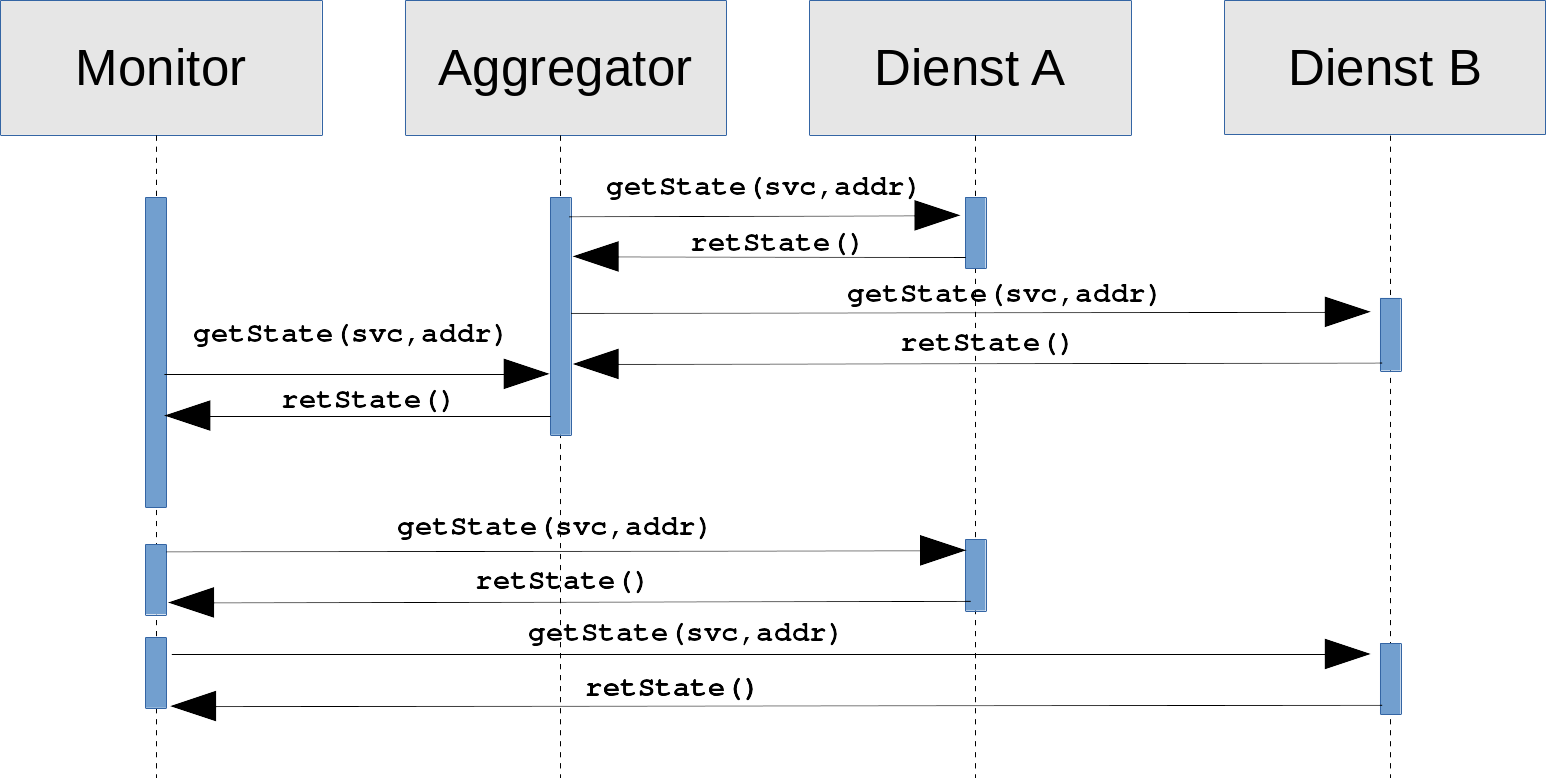
\includegraphics[scale=0.36]{img/sequence_uml_active_trans}

\end{figure}

Obiges Sequenzdiagramm (Abbildung \ref{aktiv}) zeigt schematisch den Ablauf von aktiver 
Überwachung. Der \emph{Monitor} ist die zentrale Instanz auf der alle zu überwachenden 
Informationen gesammelt, aufbereitet und ausgegeben werden. Jedoch muss der 
\emph{Monitor} nicht alle Informationen sammeln, es können auch hierarchisch 
untergeordnete 
\emph{Aggregatoren} existieren, welche ebenfalls Informationen von verschiedenen Diensten 
erheben. Diese \emph{Aggregatoren} können aus Leistungsgründen vor einen \emph{Monitor} 
geschaltet werden, um die Anzahl an abzufragenden Diensten für den \emph{Monitor} zu 
verringern. In diesem Fall bereitet bereits der \emph{Aggregator} die Daten auf und der 
\emph{Monitor} fragt nur noch die schon konsolidierten Informationen ab. Aber auch 
Segmentierungen von Infrastruktur können diesen Aufbau notwendig machen, wenn z.B. 
der \emph{Monitor} \emph{Dienst A} und \emph{Dienst B} nicht direkt erreichen kann oder 
darf. 
Zur Klassifizierung von Ereignissen werden in Überwachungslösungen\footnote{zum Beispiel: 
Nagios, Icinga} oft verschiedene Status verwendet, dies dient hauptsächlich zum 
schnelleren Verständnis für die auswertende Person. Aus diesem Grund wurden in 
Abbildung \ref{aktiv} die Bezeichnungen für der Abfragefunktionen \texttt{getState()} und 
\texttt{retState()} gewählt. Mögliche Status für die Rückgabe sind in Tabelle 
\ref{table:status} aufgeführt.

\begin{table}[ht]
    \caption{Statusübersicht}
    \label{table:status}\vspace{0.2cm}
    \centering{
    \renewcommand{\arraystretch}{1.3}
    
    \begin{tabular}{|l|l|}
        
        \hline
       \rowcolor{gray!40} \textbf{Statusbezeichnung} & \textbf{Statusbeschreibung}\\
        \hline
        \texttt{OK} & Dienst läuft innerhalb normaler Parameter.\\
        \texttt{WARNING}& Die (zuvor definierte) Warnschwelle wurde überschritten.\\
        \texttt{CRITICAL}& Die kritische Schwelle wurde überschritten oder es gab einen
        Timeout.\\
        \texttt{UNKNOWN}& Ein undefinierter Wert wurde an \emph{Monitor} übermittelt.\\
        \hline
    \end{tabular}
}

\end{table}
Ein Visualisierungsbeispiel für einen Statusverlauf eines überwachten Dienstes befindet 
sich im Anhang (Abbildung \ref{app:nag}).

\newpage
Mithilfe der Techniken zur aktiven Überwachung lassen sich zwei Klassen überwachbarer 
Dienste identifizieren: Die Betriebssystemabhängigen und die Betriebssystemunabhängigen 
Dienste. Tabelle \ref{table:aktiv} listet einige Beispiele für die jeweilige Klasse auf.


     
\begin{table}[ht]
\caption{Beispiele für aktive Überwachung}
\label{table:aktiv}\vspace{0.2cm}
\centering{
\renewcommand{\arraystretch}{1.3}
\begin{tabular}{|l|l|}
    \hline
    \rowcolor{gray!40}\textbf{Dienst / Entität }& \textbf{Beispiel} \\
    \hline
    \multicolumn{2}{|l|}{\cellcolor{shadecolor}\textbf{Betriebssystemabhängig}}\\
    \hline
    Auslastung & wie viel CPU-Zeit benötigt ein bestimmter Prozess/das ganze System\\
    Speicher & Speicherauslastung des Systems/ Belegung persistenter Speicher\\
    Prozesse & läuft ein bestimmter Prozess/ wie viele Prozesse eines Namens laufen\\
    Datendurchsatz & wie viele Bytes passieren ein Interface, Anzahl an
    \emph{paket-drops}, \emph{rejects}\\
    Audit & wurden Zugriffsregeln verletzt/ welcher Nutzer hat auf Datei X zugegriffen\\
    \hline
    \multicolumn{2}{|l|}{\cellcolor{shadecolor}\textbf{Betriebssystemunabhängig}}\\
    \hline
    \texttt{ICMP} & Netzwerkschnittstelle/ System erreichbar, \emph{round trip 
    time}\\
    \texttt{TCP/UDP} & ist bestimmter \emph{port} erreichbar\\
    Anwendungsprotokolle & Login möglich / Referenzdaten abrufbar / Rückgabewerte 
    Testroutinen\\
    \texttt{SNMP} & Abfrage beliebiger und 
    zum Teil standardisierter Messwerte\\
    \hline
\end{tabular}


}
\end{table}

\subsection{Passive Überwachung}
\begin{figure}[htbp]
    \caption{Passive Überwachung}
    \label{passiv}\vspace{0.2cm}
    \centering
    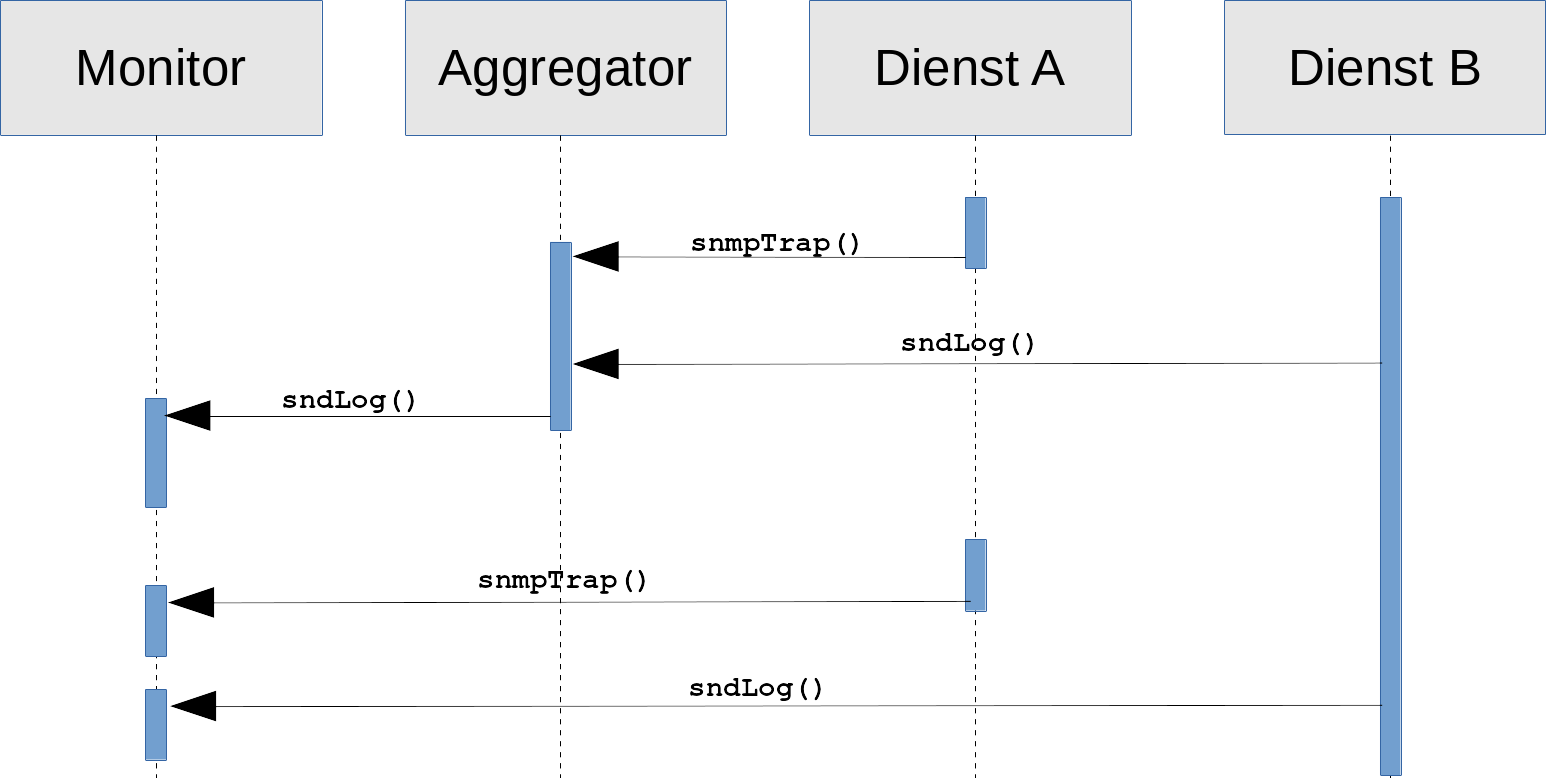
\includegraphics[scale=0.36]{img/sequence_uml_passive_trans}

\end{figure}

Wie in Abbildung \ref{passiv} zu erkennen, werden bei der passiven Überwachung nur Daten
ausgewertet, welche durch Dienste selbst generiert werden oder aber durch eine Software, 
welche den Dienst lokal überwacht. Es erfolgt keine Abfrage bei den Diensten. Der 
zentrale Punkt, welcher auch die Auswertung übernimmt, bleibt passiv und empfängt 
lediglich Meldungen. Am häufigsten sind diese Meldungen LOG-Meldungen, generiert von 
einem LOG-System. Aber auch SNMP\footnote{Simple Network Management Protocol: 
Ermöglicht eine plattformunabhängige Überwachung verschiedenster 
Endgeräte.}-Traps\footnote{SNMP-Trap: aktive Benachrichtigung des Monitors durch ein 
Endgerät/Dienst.} fallen unter diese Kategorie, daher auch die Wahl der 
Funktionsbezeichner in Abbildung \ref{passiv}.